\documentclass{article} % For LaTeX2e
\usepackage{iclr2019_conference,times}

%%%%% NEW MATH DEFINITIONS %%%%%

\usepackage{amsmath,amsfonts,bm}

% Mark sections of captions for referring to divisions of figures
\newcommand{\figleft}{{\em (Left)}}
\newcommand{\figcenter}{{\em (Center)}}
\newcommand{\figright}{{\em (Right)}}
\newcommand{\figtop}{{\em (Top)}}
\newcommand{\figbottom}{{\em (Bottom)}}
\newcommand{\captiona}{{\em (a)}}
\newcommand{\captionb}{{\em (b)}}
\newcommand{\captionc}{{\em (c)}}
\newcommand{\captiond}{{\em (d)}}

% Highlight a newly defined term
\newcommand{\newterm}[1]{{\bf #1}}


% Figure reference, lower-case.
\def\figref#1{figure~\ref{#1}}
% Figure reference, capital. For start of sentence
\def\Figref#1{Figure~\ref{#1}}
\def\twofigref#1#2{figures \ref{#1} and \ref{#2}}
\def\quadfigref#1#2#3#4{figures \ref{#1}, \ref{#2}, \ref{#3} and \ref{#4}}
% Section reference, lower-case.
\def\secref#1{section~\ref{#1}}
% Section reference, capital.
\def\Secref#1{Section~\ref{#1}}
% Reference to two sections.
\def\twosecrefs#1#2{sections \ref{#1} and \ref{#2}}
% Reference to three sections.
\def\secrefs#1#2#3{sections \ref{#1}, \ref{#2} and \ref{#3}}
% Reference to an equation, lower-case.
\def\eqref#1{equation~\ref{#1}}
% Reference to an equation, upper case
\def\Eqref#1{Equation~\ref{#1}}
% A raw reference to an equation---avoid using if possible
\def\plaineqref#1{\ref{#1}}
% Reference to a chapter, lower-case.
\def\chapref#1{chapter~\ref{#1}}
% Reference to an equation, upper case.
\def\Chapref#1{Chapter~\ref{#1}}
% Reference to a range of chapters
\def\rangechapref#1#2{chapters\ref{#1}--\ref{#2}}
% Reference to an algorithm, lower-case.
\def\algref#1{algorithm~\ref{#1}}
% Reference to an algorithm, upper case.
\def\Algref#1{Algorithm~\ref{#1}}
\def\twoalgref#1#2{algorithms \ref{#1} and \ref{#2}}
\def\Twoalgref#1#2{Algorithms \ref{#1} and \ref{#2}}
% Reference to a part, lower case
\def\partref#1{part~\ref{#1}}
% Reference to a part, upper case
\def\Partref#1{Part~\ref{#1}}
\def\twopartref#1#2{parts \ref{#1} and \ref{#2}}

\def\ceil#1{\lceil #1 \rceil}
\def\floor#1{\lfloor #1 \rfloor}
\def\1{\bm{1}}
\newcommand{\train}{\mathcal{D}}
\newcommand{\valid}{\mathcal{D_{\mathrm{valid}}}}
\newcommand{\test}{\mathcal{D_{\mathrm{test}}}}

\def\eps{{\epsilon}}


% Random variables
\def\reta{{\textnormal{$\eta$}}}
\def\ra{{\textnormal{a}}}
\def\rb{{\textnormal{b}}}
\def\rc{{\textnormal{c}}}
\def\rd{{\textnormal{d}}}
\def\re{{\textnormal{e}}}
\def\rf{{\textnormal{f}}}
\def\rg{{\textnormal{g}}}
\def\rh{{\textnormal{h}}}
\def\ri{{\textnormal{i}}}
\def\rj{{\textnormal{j}}}
\def\rk{{\textnormal{k}}}
\def\rl{{\textnormal{l}}}
% rm is already a command, just don't name any random variables m
\def\rn{{\textnormal{n}}}
\def\ro{{\textnormal{o}}}
\def\rp{{\textnormal{p}}}
\def\rq{{\textnormal{q}}}
\def\rr{{\textnormal{r}}}
\def\rs{{\textnormal{s}}}
\def\rt{{\textnormal{t}}}
\def\ru{{\textnormal{u}}}
\def\rv{{\textnormal{v}}}
\def\rw{{\textnormal{w}}}
\def\rx{{\textnormal{x}}}
\def\ry{{\textnormal{y}}}
\def\rz{{\textnormal{z}}}

% Random vectors
\def\rvepsilon{{\mathbf{\epsilon}}}
\def\rvtheta{{\mathbf{\theta}}}
\def\rva{{\mathbf{a}}}
\def\rvb{{\mathbf{b}}}
\def\rvc{{\mathbf{c}}}
\def\rvd{{\mathbf{d}}}
\def\rve{{\mathbf{e}}}
\def\rvf{{\mathbf{f}}}
\def\rvg{{\mathbf{g}}}
\def\rvh{{\mathbf{h}}}
\def\rvu{{\mathbf{i}}}
\def\rvj{{\mathbf{j}}}
\def\rvk{{\mathbf{k}}}
\def\rvl{{\mathbf{l}}}
\def\rvm{{\mathbf{m}}}
\def\rvn{{\mathbf{n}}}
\def\rvo{{\mathbf{o}}}
\def\rvp{{\mathbf{p}}}
\def\rvq{{\mathbf{q}}}
\def\rvr{{\mathbf{r}}}
\def\rvs{{\mathbf{s}}}
\def\rvt{{\mathbf{t}}}
\def\rvu{{\mathbf{u}}}
\def\rvv{{\mathbf{v}}}
\def\rvw{{\mathbf{w}}}
\def\rvx{{\mathbf{x}}}
\def\rvy{{\mathbf{y}}}
\def\rvz{{\mathbf{z}}}

% Elements of random vectors
\def\erva{{\textnormal{a}}}
\def\ervb{{\textnormal{b}}}
\def\ervc{{\textnormal{c}}}
\def\ervd{{\textnormal{d}}}
\def\erve{{\textnormal{e}}}
\def\ervf{{\textnormal{f}}}
\def\ervg{{\textnormal{g}}}
\def\ervh{{\textnormal{h}}}
\def\ervi{{\textnormal{i}}}
\def\ervj{{\textnormal{j}}}
\def\ervk{{\textnormal{k}}}
\def\ervl{{\textnormal{l}}}
\def\ervm{{\textnormal{m}}}
\def\ervn{{\textnormal{n}}}
\def\ervo{{\textnormal{o}}}
\def\ervp{{\textnormal{p}}}
\def\ervq{{\textnormal{q}}}
\def\ervr{{\textnormal{r}}}
\def\ervs{{\textnormal{s}}}
\def\ervt{{\textnormal{t}}}
\def\ervu{{\textnormal{u}}}
\def\ervv{{\textnormal{v}}}
\def\ervw{{\textnormal{w}}}
\def\ervx{{\textnormal{x}}}
\def\ervy{{\textnormal{y}}}
\def\ervz{{\textnormal{z}}}

% Random matrices
\def\rmA{{\mathbf{A}}}
\def\rmB{{\mathbf{B}}}
\def\rmC{{\mathbf{C}}}
\def\rmD{{\mathbf{D}}}
\def\rmE{{\mathbf{E}}}
\def\rmF{{\mathbf{F}}}
\def\rmG{{\mathbf{G}}}
\def\rmH{{\mathbf{H}}}
\def\rmI{{\mathbf{I}}}
\def\rmJ{{\mathbf{J}}}
\def\rmK{{\mathbf{K}}}
\def\rmL{{\mathbf{L}}}
\def\rmM{{\mathbf{M}}}
\def\rmN{{\mathbf{N}}}
\def\rmO{{\mathbf{O}}}
\def\rmP{{\mathbf{P}}}
\def\rmQ{{\mathbf{Q}}}
\def\rmR{{\mathbf{R}}}
\def\rmS{{\mathbf{S}}}
\def\rmT{{\mathbf{T}}}
\def\rmU{{\mathbf{U}}}
\def\rmV{{\mathbf{V}}}
\def\rmW{{\mathbf{W}}}
\def\rmX{{\mathbf{X}}}
\def\rmY{{\mathbf{Y}}}
\def\rmZ{{\mathbf{Z}}}

% Elements of random matrices
\def\ermA{{\textnormal{A}}}
\def\ermB{{\textnormal{B}}}
\def\ermC{{\textnormal{C}}}
\def\ermD{{\textnormal{D}}}
\def\ermE{{\textnormal{E}}}
\def\ermF{{\textnormal{F}}}
\def\ermG{{\textnormal{G}}}
\def\ermH{{\textnormal{H}}}
\def\ermI{{\textnormal{I}}}
\def\ermJ{{\textnormal{J}}}
\def\ermK{{\textnormal{K}}}
\def\ermL{{\textnormal{L}}}
\def\ermM{{\textnormal{M}}}
\def\ermN{{\textnormal{N}}}
\def\ermO{{\textnormal{O}}}
\def\ermP{{\textnormal{P}}}
\def\ermQ{{\textnormal{Q}}}
\def\ermR{{\textnormal{R}}}
\def\ermS{{\textnormal{S}}}
\def\ermT{{\textnormal{T}}}
\def\ermU{{\textnormal{U}}}
\def\ermV{{\textnormal{V}}}
\def\ermW{{\textnormal{W}}}
\def\ermX{{\textnormal{X}}}
\def\ermY{{\textnormal{Y}}}
\def\ermZ{{\textnormal{Z}}}

% Vectors
\def\vzero{{\bm{0}}}
\def\vone{{\bm{1}}}
\def\vmu{{\bm{\mu}}}
\def\vtheta{{\bm{\theta}}}
\def\va{{\bm{a}}}
\def\vb{{\bm{b}}}
\def\vc{{\bm{c}}}
\def\vd{{\bm{d}}}
\def\ve{{\bm{e}}}
\def\vf{{\bm{f}}}
\def\vg{{\bm{g}}}
\def\vh{{\bm{h}}}
\def\vi{{\bm{i}}}
\def\vj{{\bm{j}}}
\def\vk{{\bm{k}}}
\def\vl{{\bm{l}}}
\def\vm{{\bm{m}}}
\def\vn{{\bm{n}}}
\def\vo{{\bm{o}}}
\def\vp{{\bm{p}}}
\def\vq{{\bm{q}}}
\def\vr{{\bm{r}}}
\def\vs{{\bm{s}}}
\def\vt{{\bm{t}}}
\def\vu{{\bm{u}}}
\def\vv{{\bm{v}}}
\def\vw{{\bm{w}}}
\def\vx{{\bm{x}}}
\def\vy{{\bm{y}}}
\def\vz{{\bm{z}}}

% Elements of vectors
\def\evalpha{{\alpha}}
\def\evbeta{{\beta}}
\def\evepsilon{{\epsilon}}
\def\evlambda{{\lambda}}
\def\evomega{{\omega}}
\def\evmu{{\mu}}
\def\evpsi{{\psi}}
\def\evsigma{{\sigma}}
\def\evtheta{{\theta}}
\def\eva{{a}}
\def\evb{{b}}
\def\evc{{c}}
\def\evd{{d}}
\def\eve{{e}}
\def\evf{{f}}
\def\evg{{g}}
\def\evh{{h}}
\def\evi{{i}}
\def\evj{{j}}
\def\evk{{k}}
\def\evl{{l}}
\def\evm{{m}}
\def\evn{{n}}
\def\evo{{o}}
\def\evp{{p}}
\def\evq{{q}}
\def\evr{{r}}
\def\evs{{s}}
\def\evt{{t}}
\def\evu{{u}}
\def\evv{{v}}
\def\evw{{w}}
\def\evx{{x}}
\def\evy{{y}}
\def\evz{{z}}

% Matrix
\def\mA{{\bm{A}}}
\def\mB{{\bm{B}}}
\def\mC{{\bm{C}}}
\def\mD{{\bm{D}}}
\def\mE{{\bm{E}}}
\def\mF{{\bm{F}}}
\def\mG{{\bm{G}}}
\def\mH{{\bm{H}}}
\def\mI{{\bm{I}}}
\def\mJ{{\bm{J}}}
\def\mK{{\bm{K}}}
\def\mL{{\bm{L}}}
\def\mM{{\bm{M}}}
\def\mN{{\bm{N}}}
\def\mO{{\bm{O}}}
\def\mP{{\bm{P}}}
\def\mQ{{\bm{Q}}}
\def\mR{{\bm{R}}}
\def\mS{{\bm{S}}}
\def\mT{{\bm{T}}}
\def\mU{{\bm{U}}}
\def\mV{{\bm{V}}}
\def\mW{{\bm{W}}}
\def\mX{{\bm{X}}}
\def\mY{{\bm{Y}}}
\def\mZ{{\bm{Z}}}
\def\mBeta{{\bm{\beta}}}
\def\mPhi{{\bm{\Phi}}}
\def\mLambda{{\bm{\Lambda}}}
\def\mSigma{{\bm{\Sigma}}}

% Tensor
\DeclareMathAlphabet{\mathsfit}{\encodingdefault}{\sfdefault}{m}{sl}
\SetMathAlphabet{\mathsfit}{bold}{\encodingdefault}{\sfdefault}{bx}{n}
\newcommand{\tens}[1]{\bm{\mathsfit{#1}}}
\def\tA{{\tens{A}}}
\def\tB{{\tens{B}}}
\def\tC{{\tens{C}}}
\def\tD{{\tens{D}}}
\def\tE{{\tens{E}}}
\def\tF{{\tens{F}}}
\def\tG{{\tens{G}}}
\def\tH{{\tens{H}}}
\def\tI{{\tens{I}}}
\def\tJ{{\tens{J}}}
\def\tK{{\tens{K}}}
\def\tL{{\tens{L}}}
\def\tM{{\tens{M}}}
\def\tN{{\tens{N}}}
\def\tO{{\tens{O}}}
\def\tP{{\tens{P}}}
\def\tQ{{\tens{Q}}}
\def\tR{{\tens{R}}}
\def\tS{{\tens{S}}}
\def\tT{{\tens{T}}}
\def\tU{{\tens{U}}}
\def\tV{{\tens{V}}}
\def\tW{{\tens{W}}}
\def\tX{{\tens{X}}}
\def\tY{{\tens{Y}}}
\def\tZ{{\tens{Z}}}


% Graph
\def\gA{{\mathcal{A}}}
\def\gB{{\mathcal{B}}}
\def\gC{{\mathcal{C}}}
\def\gD{{\mathcal{D}}}
\def\gE{{\mathcal{E}}}
\def\gF{{\mathcal{F}}}
\def\gG{{\mathcal{G}}}
\def\gH{{\mathcal{H}}}
\def\gI{{\mathcal{I}}}
\def\gJ{{\mathcal{J}}}
\def\gK{{\mathcal{K}}}
\def\gL{{\mathcal{L}}}
\def\gM{{\mathcal{M}}}
\def\gN{{\mathcal{N}}}
\def\gO{{\mathcal{O}}}
\def\gP{{\mathcal{P}}}
\def\gQ{{\mathcal{Q}}}
\def\gR{{\mathcal{R}}}
\def\gS{{\mathcal{S}}}
\def\gT{{\mathcal{T}}}
\def\gU{{\mathcal{U}}}
\def\gV{{\mathcal{V}}}
\def\gW{{\mathcal{W}}}
\def\gX{{\mathcal{X}}}
\def\gY{{\mathcal{Y}}}
\def\gZ{{\mathcal{Z}}}

% Sets
\def\sA{{\mathbb{A}}}
\def\sB{{\mathbb{B}}}
\def\sC{{\mathbb{C}}}
\def\sD{{\mathbb{D}}}
% Don't use a set called E, because this would be the same as our symbol
% for expectation.
\def\sF{{\mathbb{F}}}
\def\sG{{\mathbb{G}}}
\def\sH{{\mathbb{H}}}
\def\sI{{\mathbb{I}}}
\def\sJ{{\mathbb{J}}}
\def\sK{{\mathbb{K}}}
\def\sL{{\mathbb{L}}}
\def\sM{{\mathbb{M}}}
\def\sN{{\mathbb{N}}}
\def\sO{{\mathbb{O}}}
\def\sP{{\mathbb{P}}}
\def\sQ{{\mathbb{Q}}}
\def\sR{{\mathbb{R}}}
\def\sS{{\mathbb{S}}}
\def\sT{{\mathbb{T}}}
\def\sU{{\mathbb{U}}}
\def\sV{{\mathbb{V}}}
\def\sW{{\mathbb{W}}}
\def\sX{{\mathbb{X}}}
\def\sY{{\mathbb{Y}}}
\def\sZ{{\mathbb{Z}}}

% Entries of a matrix
\def\emLambda{{\Lambda}}
\def\emA{{A}}
\def\emB{{B}}
\def\emC{{C}}
\def\emD{{D}}
\def\emE{{E}}
\def\emF{{F}}
\def\emG{{G}}
\def\emH{{H}}
\def\emI{{I}}
\def\emJ{{J}}
\def\emK{{K}}
\def\emL{{L}}
\def\emM{{M}}
\def\emN{{N}}
\def\emO{{O}}
\def\emP{{P}}
\def\emQ{{Q}}
\def\emR{{R}}
\def\emS{{S}}
\def\emT{{T}}
\def\emU{{U}}
\def\emV{{V}}
\def\emW{{W}}
\def\emX{{X}}
\def\emY{{Y}}
\def\emZ{{Z}}
\def\emSigma{{\Sigma}}

% entries of a tensor
% Same font as tensor, without \bm wrapper
\newcommand{\etens}[1]{\mathsfit{#1}}
\def\etLambda{{\etens{\Lambda}}}
\def\etA{{\etens{A}}}
\def\etB{{\etens{B}}}
\def\etC{{\etens{C}}}
\def\etD{{\etens{D}}}
\def\etE{{\etens{E}}}
\def\etF{{\etens{F}}}
\def\etG{{\etens{G}}}
\def\etH{{\etens{H}}}
\def\etI{{\etens{I}}}
\def\etJ{{\etens{J}}}
\def\etK{{\etens{K}}}
\def\etL{{\etens{L}}}
\def\etM{{\etens{M}}}
\def\etN{{\etens{N}}}
\def\etO{{\etens{O}}}
\def\etP{{\etens{P}}}
\def\etQ{{\etens{Q}}}
\def\etR{{\etens{R}}}
\def\etS{{\etens{S}}}
\def\etT{{\etens{T}}}
\def\etU{{\etens{U}}}
\def\etV{{\etens{V}}}
\def\etW{{\etens{W}}}
\def\etX{{\etens{X}}}
\def\etY{{\etens{Y}}}
\def\etZ{{\etens{Z}}}

% The true underlying data generating distribution
\newcommand{\pdata}{p_{\rm{data}}}
% The empirical distribution defined by the training set
\newcommand{\ptrain}{\hat{p}_{\rm{data}}}
\newcommand{\Ptrain}{\hat{P}_{\rm{data}}}
% The model distribution
\newcommand{\pmodel}{p_{\rm{model}}}
\newcommand{\Pmodel}{P_{\rm{model}}}
\newcommand{\ptildemodel}{\tilde{p}_{\rm{model}}}
% Stochastic autoencoder distributions
\newcommand{\pencode}{p_{\rm{encoder}}}
\newcommand{\pdecode}{p_{\rm{decoder}}}
\newcommand{\precons}{p_{\rm{reconstruct}}}

\newcommand{\laplace}{\mathrm{Laplace}} % Laplace distribution

\newcommand{\E}{\mathbb{E}}
\newcommand{\Ls}{\mathcal{L}}
\newcommand{\R}{\mathbb{R}}
\newcommand{\emp}{\tilde{p}}
\newcommand{\lr}{\alpha}
\newcommand{\reg}{\lambda}
\newcommand{\rect}{\mathrm{rectifier}}
\newcommand{\softmax}{\mathrm{softmax}}
\newcommand{\sigmoid}{\sigma}
\newcommand{\softplus}{\zeta}
\newcommand{\KL}{D_{\mathrm{KL}}}
\newcommand{\Var}{\mathrm{Var}}
\newcommand{\standarderror}{\mathrm{SE}}
\newcommand{\Cov}{\mathrm{Cov}}
% Wolfram Mathworld says $L^2$ is for function spaces and $\ell^2$ is for vectors
% But then they seem to use $L^2$ for vectors throughout the site, and so does
% wikipedia.
\newcommand{\normlzero}{L^0}
\newcommand{\normlone}{L^1}
\newcommand{\normltwo}{L^2}
\newcommand{\normlp}{L^p}
\newcommand{\normmax}{L^\infty}

\newcommand{\parents}{Pa} % See usage in notation.tex. Chosen to match Daphne's book.

\DeclareMathOperator*{\argmax}{arg\,max}
\DeclareMathOperator*{\argmin}{arg\,min}

\DeclareMathOperator{\sign}{sign}
\DeclareMathOperator{\Tr}{Tr}
\let\ab\allowbreak


\usepackage{hyperref}
\usepackage{url}
\usepackage[encapsulated]{CJK}
\usepackage{graphicx}


\title{CS Tacotron: \\ End-to-End Chinese-English Code-Switching Speech Synthesis on the LectureDSP Dataset}

\author{Ting-Wei Liu, Tao Tu \\
Speech Lab 531\\
National Taiwan University\\
\texttt{\{R07942089,R07922022\}@ntu.edu.tw} \\
}

\newcommand{\fix}{\marginpar{FIX}}
\newcommand{\new}{\marginpar{NEW}}

\iclrfinalcopy % Uncomment for camera-ready version, but NOT for submission.

\begin{document}
\begin{CJK}{UTF8}{bsmi}


\maketitle
\begin{abstract}
With the wide success of recent machine learning Text-to-speech (TTS)  models, promising results on synthesizing realistic speech have proven machine's capability of synthesizing human-like voices. However, little progress has been made in the domain of Chinese-English code-switching text-to-speech synthesis, where machine has to learn to handle both input and output in a multilingual fashion. In this work, we present Code-Switch Tacotron, which is built based on the state-of-the-art end-to-end  text-to-speech generative model~\citep{Wang2017}. CS-Tacotron is capable of synthesizing code-switching speech conditioned on raw CS text. Given CS text and audio pairs, our model can be trained end-to-end  with proper data pre-processing. Furthurmore, we train our model on the LectureDSP dataset, a Chinese-English code-switching lecture-based dataset, which originates from the course Digital Signal Processing (DSP) offered in National Taiwan University (NTU). We present several key implementation techniques to make the Tacotron model perform well on this challenging multilingual speech generation task. In addition, we present a demo system, which demonstrates the  Chinese-English code-switching speech synthesis results of our model. CS-Tacotron possess the capability of  generating CS speech from CS text, and speaks vividly with the style of LectureDSP's speaker.
\end{abstract}

\section{Introduction}

Modern end-to-end TTS systems have many well known advantages when compared to antique TTS pipelines such as statistical parametric TTS systems. In parametric TTS, speech synthesis are achieved through the composition of multiple components: a text processor which extracts various linguistic features, a duration model, an acoustic feature prediction model, and a complex signal-processing-based vocoder. All of which requires significant amount of domain knowledge and complex design, building such systems consumes substantial engineering efforts. More over, the combination of these components leads to more error, as they are all trained separately. However an end-to-end TTS can be trained on raw text and audio pairs, in which a single model covers all the components in statistical parametric TTS system's multi-stage model. In this work, we incorporate Tacotron~\citep{Wang2017}, an end-to-end generative TTS model based on sequence-to-sequence~\citep{Sutskever2014} with attention~\citep{Bahdanau2014}. Tacotron achieves an outstanding performance when trained and tested on monolingual English data, as reported by \citet{Wang2017}. The many advantages of an end-to-end model, makes adaptation of such model to a new type of code-switching data tractable. With the success of Tacotron, we further tackle the problem of Chinese-English code-switching speech synthesis.

Reports reveal that people communicates in code-switching languages in everyday life~\citep{Nakayama12018}, since modern people may not always communicate in monolingual settings, spoken language technologies such as TTS must be developed to handle multilingual input and output. The original TTS transforms highly compressed source (text) into diversely decompressed result (audio). Since the same text can correspond to different pronunciations or styles, this is a particularly difficult learning task for an end-to-end model. In the case of CS TTS, the model has to cope with an even larger output variation for a given input, as two languages are now mixed together. Not only do pronunciations varies between language and language, the input is also entangled with multilingual units. This results in a large-scale inverse mapping problem: mapping highly compact Chinese-English code-switching text to human-like Chinese-English code-switching speech. \citet{Liang2007} attempted to solve the Chinese-English switching language problem and proposed context-dependent HMM state sharing for their code-switched TTS system, which in this work we address the problem with an alternative approach: an end-to-end neural net model instead of HMM. Despite extensive studies on bilingual spoken language technologies, the Chinese-English code-switching case remains a scant research topic up to now, mainly due to the lack of quality and quantity of Chinese-English text audio parallel data.

Combining the two problems of text-to-speech synthesis and code-switching, in this work we present our solution: CS-Tacotron, a sequence-to-sequence based model with attention built upon the successful work of \citet{Wang2017}, together with LectureDSP, a diverse and rich Chinese-English code-switching dataset that contains parallel CS text and audio. The model takes Chinese-English mixed text as input, and outputs predicted spectrograms conditioned on the input text. We use the Griffin-Lim Algorithm~\citep{Griffin11984} to perform fast waveform synthesis from spectral magnitude sampled on a linear-frequency scale. To handle both Chinese and English text inputs, we use English characters as subword linguistic units for our model's input. Given raw CS text and audio pairs, our data pre-processing pipeline allows the model to be trained completely from random initialization. It does not require further human effort to label phoneme-level alignment, so it can easily scale to using other datasets that contains acoustic data with transcripts. As a result, the presented CS-Tacotron is capable of handling multilingual Chinese-English input and generates human-like code-switching speech accordingly. We claim that it is the implementation details and tricks that makes the migration of monolingual Tacotron~\citep{Wang2017} to multilingual CS-Tacotron successful, we present our key contributions in the following sections.

\section{Dataset - LectureDSP}
Parallel transcripts and speech of code-switching data are extremely rare and valuable, the LectureDSP originates from the Digital Signal Processing (DSP) course offered in National Taiwan University (NTU), which is also available online: \url{http://speech.ee.ntu.edu.tw/}. The course DSP is offered by professor Lin-Shan Lee from the Department of Electrical Engineering and Department of Computer Science and Information Engineering in NTU. Chinese-English code-switching lecture speech are recorded and segmented into sentences, with proper multilingual transcripts labeled by human annotation, resulting in a well organized parallel text and audio Chinese-English dataset. We take no credit for the collection and organization of the LectureDSP dataset, it was processed by former members of the NTU Speech Lab. Currently this dataset is not available for public release and remains a private collection in the lab.

\subsection{Details and Analysis}
LectureDSP is a lecture-based speech dataset, containing over 13700 short audio clips of a single  male speaker giving lectures in a university course. The domain of LectureDSP's content covers general greetings, daily conversations, and technological terms in the field of digital speech processing (DSP). A transcription is provided for each audio clip, clips vary in length from 1 to 18 seconds, with an average length of 3.6 seconds, and a total length of approximately 13.7 hours. We calculate the average code-switching frequency throughout the dataset to be 974 switches per hour in average. Where we consider the use of a English vocabulary to be a switch, the total number of switch is 13346 throughout the dataset, and the number of sentences that contains a switch is 6506 (out of a total of 13720). The speech recordings were conducted in an open space (classroom) using a microphone, which introduce considerable noise in speech quality. The quality of training data can be considered as an upper bound of speech generation quality, in this work we also use this dataset to measure the goodness of our model.

\subsection{Transcript Pre-processing}
The original transcripts in LectureDSP were consists of a mix of English vocabularies and big5 character codes, these 4 digit codes represents Chinese characters in a one to one mapping relation. We use a code-to-character mapping table (\url{http://ash.jp/code/cn/big5tbl.htm}) to covert the 4 digit codes into Chinese characters. For example, the original transcript "OKAY [A66E] [A655][A6EC] [A6AD]" will be converted to "OKAY 好 各位 早". We process all transcripts and obtain a new set of sentences that consist of a mix of English words and Chinese characters. These sentences are then converted to Chinese pinyin using the Python PyPinYin(\url{https://pypi.org/project/pypinyin/} toolkit. For example the Chinese character "中心" will be converted to "zhong xin", this also is a one-to-one mapping. Now we can treat all inputs as a sequence of English characters (letters), we compressed the large vocabulary dimension of Chinese characters into just only 26 English letters (a-z). However, we found that for successful training and generation, we need to distinguish English letter sequences and Chinese pinyin letter sequences with upper case and lower case letters, respectively. As a result, our model handles the following input tokens: 26 lower case English letters (a-z), 26 upper case English letters (A-Z) and three special tags ([bos], [eos], [spc]) that denote the start and end of sentences, and the spaces between words.

\subsection{Speech Pre-processing}
Since LectureDSP contains the speech of a single male speaker, and we know that male voice covers a frequency range of 100Hz to 8KHz, and a microphone range (300 Hz-3.4 kHz) has okay intelligibility but the quality of the voice is fairly compromised. Hence we decide cut off the frequencies below 100Hz by a high-pass filter to remove unwanted noise, and smooth out the frequencies ranging from 100Hz to 300Hz. Furthermore, we normalize the volume of the entire dataset to -10 dB for volume consistency. In Figure 1, we show a sample drawn from the dataset, showing the differences between the pre-processed waveform (above) and the original waveform (below). We found that the simple speech pre-processing scheme we used did help improve the quality of LectureDSP, and we train our model on the processed waveform for better generation quality.
\begin{figure}[h]
\begin{center}
\fbox{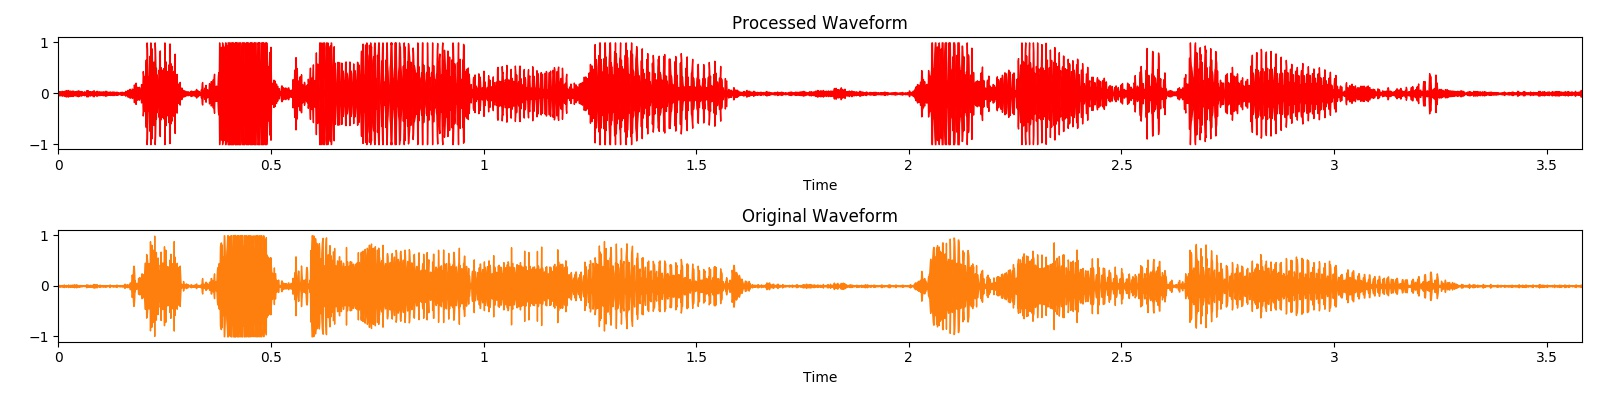
\includegraphics[scale=0.337]{images/speech_preprocess.jpeg}}
\end{center}
\caption{Speech Pre-processing Comparison}
\end{figure}

\section{Model Implementation}
The TTS model we used is based on the sequence-to-sequence Tacotron by \citet{Wang2017}, where we further modify some architectures and apply several implementation tricks. In this section, we described the main differences of our model from the original work, we believe that these implementation details are crucial to our success. We predict r=5 non-overlapping consecutive output frames at each decoder step instead of r=2, this divides the total number of decoder steps by r, which reduces model size, training time, and inference time. Additionally, we feed all r frames to the next decoder step for the sequence-to-sequence input instead of just the last frame in r frames. The post-processing net’s task is to convert the seq2seq target (r frames) to linear-scale spectrogram, we scale the loss on these spectrogram so that lower frequencies that corresponds to human speech (0 to 3000 Hz) weighs more. The reason for this modification is that this loss adjustment makes the model attend more on the crucial frequency band of human speech, to be specific we use a weighting of 0.5 * loss(0-3000Hz) + 0.5 * loss(other frequencies) on linear-scale spectrogram loss. We did not use a loss mask in the sequence-to-sequence learning problem, which means we count the loss for all padding, this forces the model to learn when to stop the synthesis sequence. We use a decaying learning rate, as proposed by \citet{Vaswani2017}, where the initial learning rate is set to 0.002. Moreover, the CBHG module in Tacotron was modified so that the 1-Dimensional convolution unit has no bias, and we did not disable pre-net's dropout during inference time, we found that the dropout increases the model's generalization for unseen inputs. With the above technological alternation, our model can be successfully trained on CS data. Training time is approximately 24 hours for the model to converge on a GeForce GTX-980 Ti machine.

\begin{figure}[h]
\begin{center}
\fbox{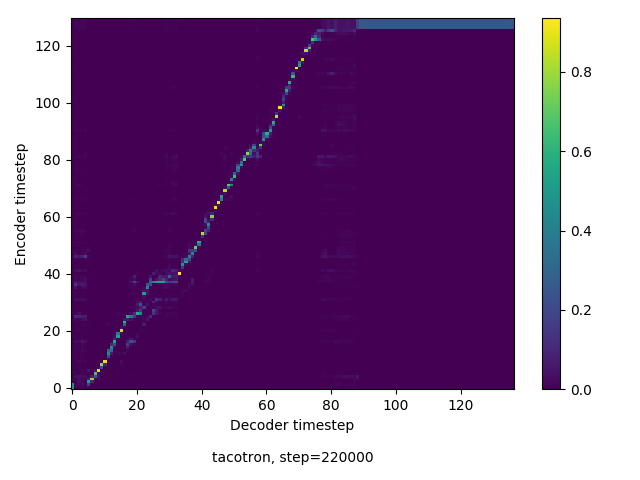
\includegraphics[scale=0.5]{images/alignment_1.png}}
\end{center}
\caption{The alignment plot with teacher forcing in training phase.}
\end{figure}

\section{Result}
At each timestep, the decoder will attend on parts of the encoder output, i.e., the text embedding , and output r (reduction factor) frames of mel-spectrogram as described by \citet{Wang2017}. In Figure 2, we show the alignment plot with teacher forcing of our model in training phase (At the 220000-th iterations). We can see that our model is capable of capturing the monotonic alignment property of the text-to-speech task. We can observe that the alignment plot contains some blurry parts, this is caused by the following two reasons: Firstly, pronouncing consecutive Chinese characters with the same pronunciation is difficult for an end-to-end model. Secondly, the training data (LectureDSP) we used is not the best to suit good TTS generation quality.  In Figure 3, we show the alignment plot of our model's testing phase, where the first is the alignment plot of monolingual Chinese input, the second is the alignment plot of Chinese-English code-switching input, and the third is monolingual English input. The inputs are: 這是數位語音處理, 這是數位語音PROCESSING, THIS IS DIGITAL SPEECH PROCESSING, respectively. We can see that our model performs well when performing full Chinese generation and code-switching synthesis, but fails to generate a sentence consists of full monolingual English. We conclude that this is because the training data contains no full English sentences, hence the model fails to generalize from sparse English words contained in Chinese-based code-switching training data. The trained model is capable of synthesizing human-like speech, with a style easily recognizable to be the speaker of the LectureDSP dataset, suggesting that our model is able to capture the style of the trained speaker. We deemed that training is successfully given that the training data is limited and the reference audio's quality  is not the best for TTS training. We present the generation quality of our model in a live demo session, however for the need of reproduction of our results we open source the code we use.

The Pytorch implementation of our work, including the trained model, training algorithms, testing algorithms, and data pre-processing scripts, is available at the following link with a detailed Readme file: \url{https://github.com/andi611/CS-Tacotron}.

\begin{figure}[h]
\begin{center}
\fbox{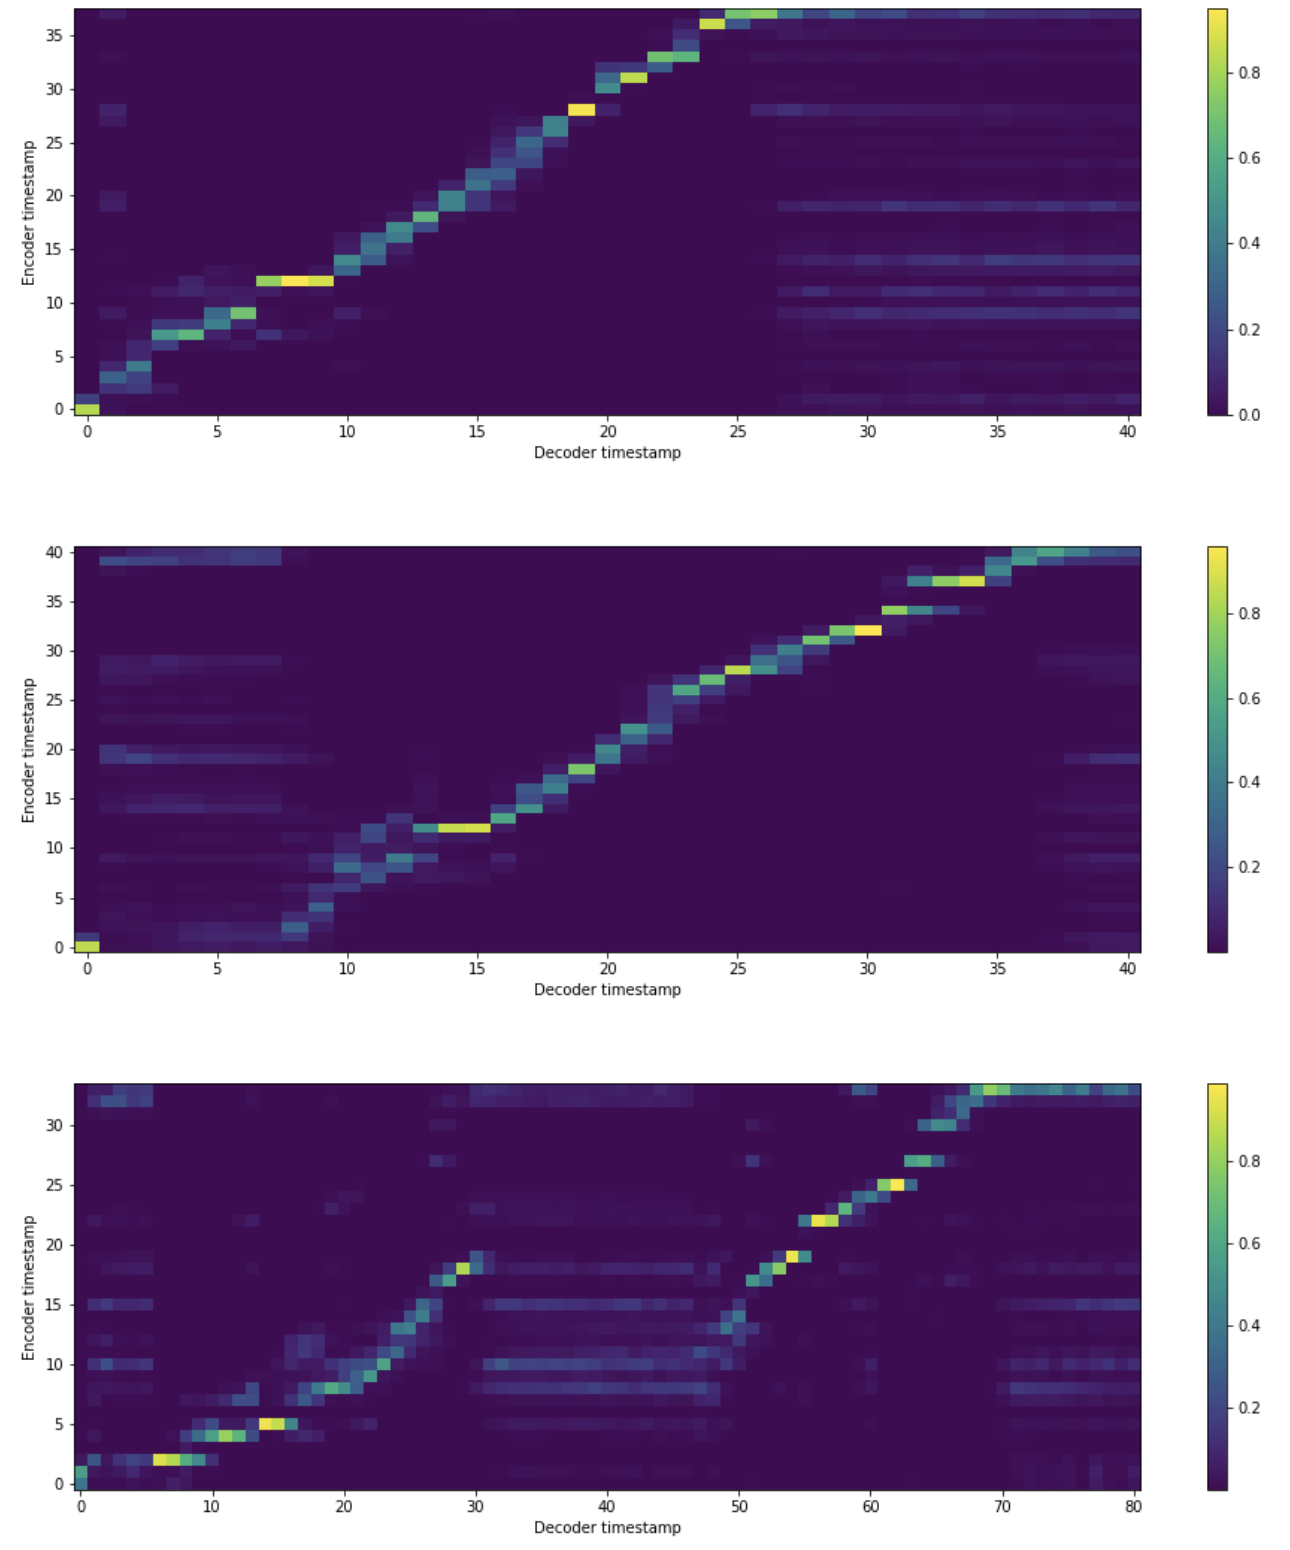
\includegraphics[scale=0.5]{images/alignment_2.png}}
\end{center}
\caption{The attention plot without teacher forcing in testing phase. The inputs are: 這是數位語音處理, 這是數位語音PROCESSING, THIS IS DIGITAL SPEECH PROCESSING, respectively.
}
\end{figure}

\section{Discussions}
We have proposed CS-Tacotron, a code-switching speech synthesis end-to-end generative TTS model based on the work of \citet{Wang2017}. Our model takes a character sequence as input, which is provided by our data pre-processing pipeline that transforms Chinese-English mixed word sequences into English character sequence. Given the pre-processed input, our model outputs the corresponding spectrogram, which is later synthesized to code-switching speech. Unlike previous work, our method does not need to handle engineered linguistic features or complex components such as a HMM. It is general and can be easily integrated to other code-switching training schemes, where in this work we prove the training of such TTS model to be successful on our own dataset LectureDSP. CS-Tacotron successfully modeled the style and code-switching fashion of the speaker, and is capable of generating reasonable and understandable speech utterances.

We have yet to investigate a larger scale model-wise modification to specifically suit the code-switching audio generation paradigm; many designs of the original Tacotron model remains unchanged. The Griffin-Lim-based waveform synthesizer is also well known to produce outputs with audible artifacts, which explains the quality of our generated audio. Future work may include model framework modification, and experimenting with different subword linguistic units for code-switching TTS models.

\subsubsection*{Acknowledgments}
The authors would like to specially thank professor Lin-Shan Lee for offering the wonderful course DSP and providing the LectureDSP dataset. Additionally we thank the members of Speech Lab for constructive discussions and feedback.

Furthermore, we would like to give credit to Ryuichi Yamamoto for this wonderful Pytorch implementation of Tacotron: \url{https://github.com/r9y9/tacotron_pytorch}, which we mainly based our work on.

\bibliography{iclr2019_conference}
\bibliographystyle{iclr2019_conference}

\end{CJK}
\end{document}